% \begin{mdframed}
%     \textbf{La extensión máxima para esta sección es de 4 páginas.} Si utiliza menos páginas y explica bien sus resultados, es preferible.
% \end{mdframed}

% Presente sus resultados mediante \textbf{tablas y gráficos}. Cada tabla o gráfico debe estar referenciado en el texto, con una breve descripción de lo que se observa y por qué es relevante.

% \textbf{Es necesario automatizar la generación de las gráficas}, ya que es imprescindible que se pueda confirmar que las visualizaciones presentadas son producto de los datos generados por sus algoritmos.

% Escoja las gráficas más representativas y que muestren de manera clara los resultados obtenidos. Esta elección es parte de lo que se evaluará en la sección de presentación de resultados.



% \begin{mdframed}
%     Recuerde que es imprescindible que se pueda replicar la generación de las gráficas, por lo que usted debe referir a las figuras generadas en `code/matrix\_multiplication/data/plots/` y `code/sorting/data/plots/`.
% \end{mdframed}


% \begin{mdframed}
%     \textbf{La extensión máxima para esta sección es de 6 páginas.}
% \end{mdframed}

Gráficos obtenidos. Los resultados se guardan como \texttt{<algoritmo>.csv} en la ruta

\path{code/<problema>/data/measurements}

Cada registro incluye tamaño de entrada, dimensión y tiempo de ejecución en ms. Para generar los datos, entrar a \path{code/<problema>/}, ejecutar \texttt{make} y luego \texttt{./<problema>}.
Los CSV quedarán en data/measurements.

Para generar las gráficas, entrar a \path{code/<problema>/scripts/} y ejecutar el comando:

\texttt{python3 plot\_generator.py}

Se requiere módulos de Python3: Pandas, NumPy, Matplotlib, Seaborn y Warnings.

\subsection*{Algoritmos de Ordenamiento}

\subsubsection*{Análisis de Tiempo}

Aquí se presentan los resultados obtenidos. La Figura 1 compara todos los algoritmos en relación con Tiempo \(ms\) y Tamaño de la entrada definidas por el enunciado del problema. Usamos la escala logarítmica para facilitar la visualización de los datos.
\begin{figure}[H]
    \centering
    \begin{minipage}[t]{0.49\textwidth}
        \centering
        % code/sorting/data/plots/01_tiempo_vs_tamaño.png
        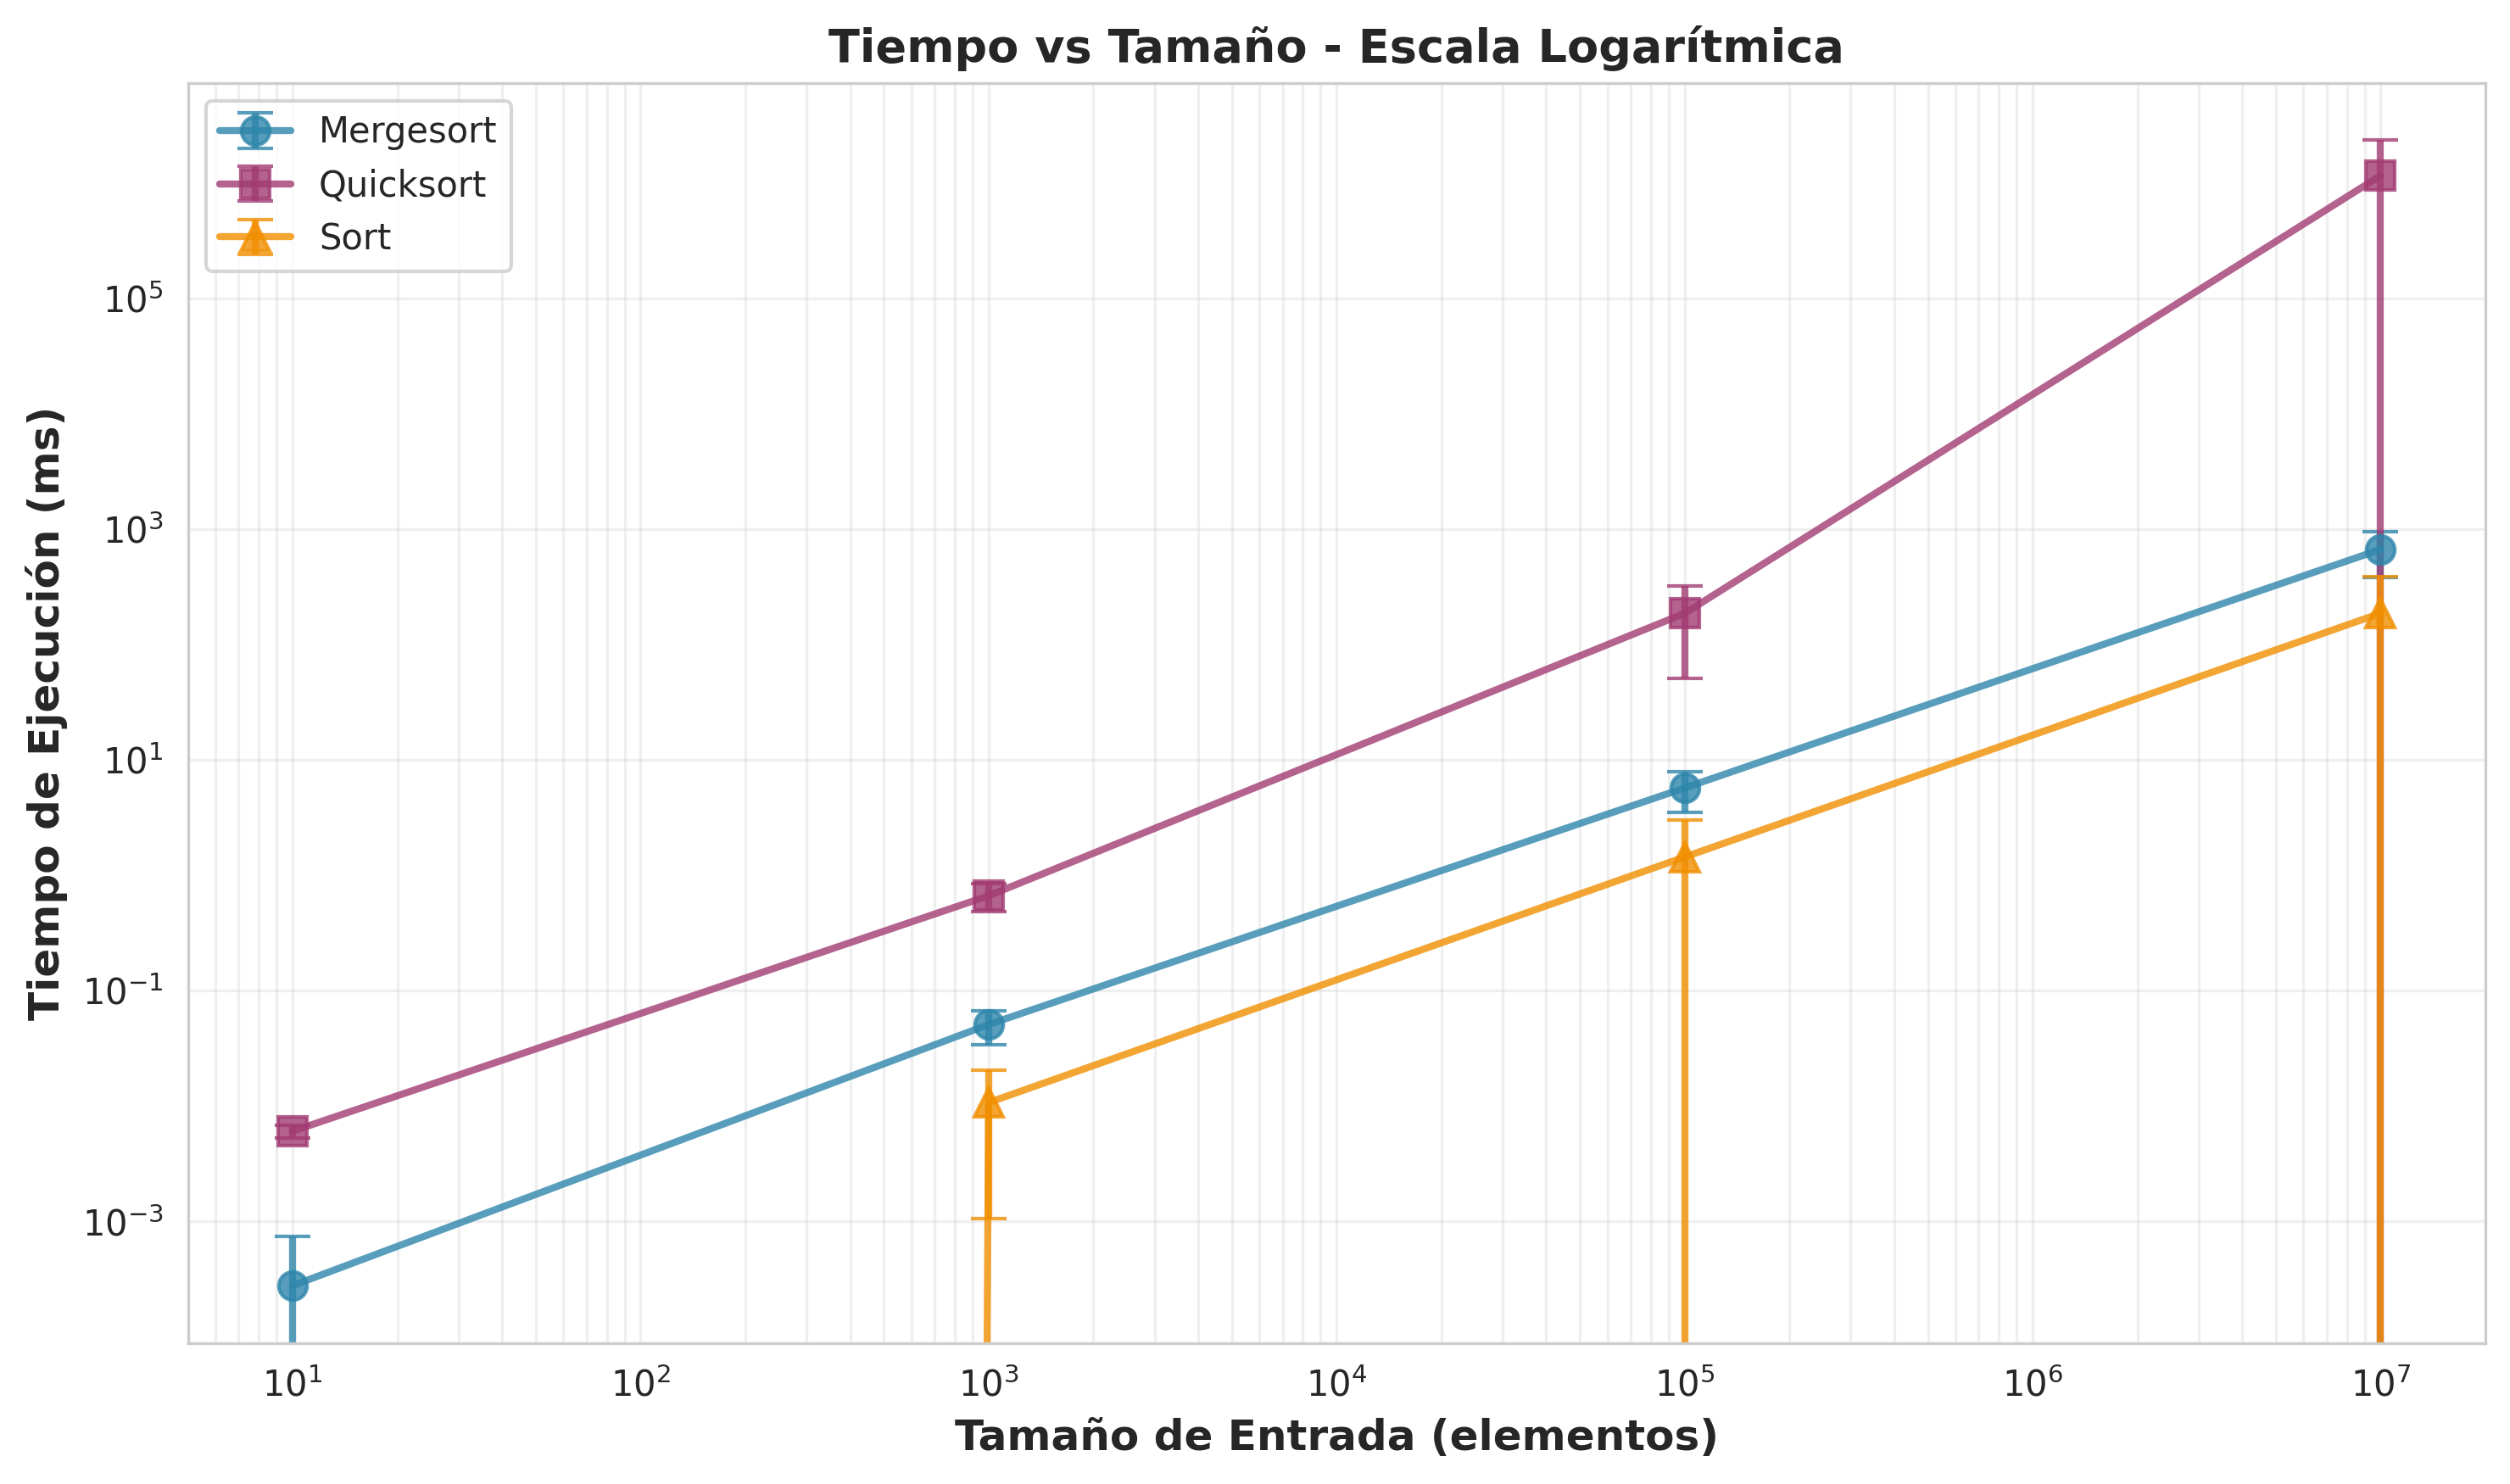
\includegraphics[width=\textwidth]{../code/sorting/data/plots/01_tiempo_vs_tamaño.png}
        \caption{Todos los algoritmos Sorts.}
    \end{minipage}
\end{figure}

\textit{El tiempo registrado de Sort para datos de tamaño menor a $10^3$ fue de 0 ms por su rapidez.}

En la \textbf{Figura 1} podemos observar nuestro segundo peor algoritmo estudiado, comenzaremos analizaremos Quick Sort, con la implementación de Random Pivot, que en teoría debería ser el mejor algoritmo gracias a su media de tiempo de $O(n * log(n))$, pero al entrar en su peor caso, que es $O(n^2)$, y al encontrar matrices de tamaño $10^7$, y gracias a las repetidas llamadas recursivas se se puede encontrar con el problema de Segmentation Fault, que significa un rebalse de la memoria Stack, por lo que puede tener problemas ejecutando un ordenamiento de tamaño $10^7$.

Después, podemos observar el Merge Sort, como lo visto en clases, este algoritmo tiene un tiempo de ejecución de $O(n * log (n))$, y es el segundo mejor algoritmo después de Sort de C++. Y claramente podemos observar su comportamiento logarítmico en la gráfica. No es el mejor, ya que en arreglos grandes, Merge Sort utilizará memoria adicional para combinar las sublistas, a diferencia de Quick Sort y Sort que son in-place.

Por último, tenemos Sort, que en la práctica es el mejor algoritmo de todos, este algoritmo está basado en Introsort, que es una combinación de 3 métodos: Quick Sort, Heap Sort y Insertion Sort. El algoritmo comienza utilizando Quick Sort y cuando detecta que la recursión es profunda cambia automáticamente a Heap Sort para evitar el peor de los casos $O(n^2)$. Por esto mismo es el mejor de todos ya que minimiza, casi anula completamente alguna chance de entrar a su peor caso, manteniendo su tiempo de ejecución en $O(n * log (n))$.

\subsubsection*{Análisis de Memoria}

En el Análisis de Memoria se muestran cuatro métricas: \textit{Delta RSS}, \textit{Peak Memory}, \textit{Delta Peak desde Inicio} y \textit{RSS Después}. Algunas métricas representan memoria total del proceso y otras representan crecimiento real debido a cómo se implementa el programa.

\begin{figure}[H]
    \centering
    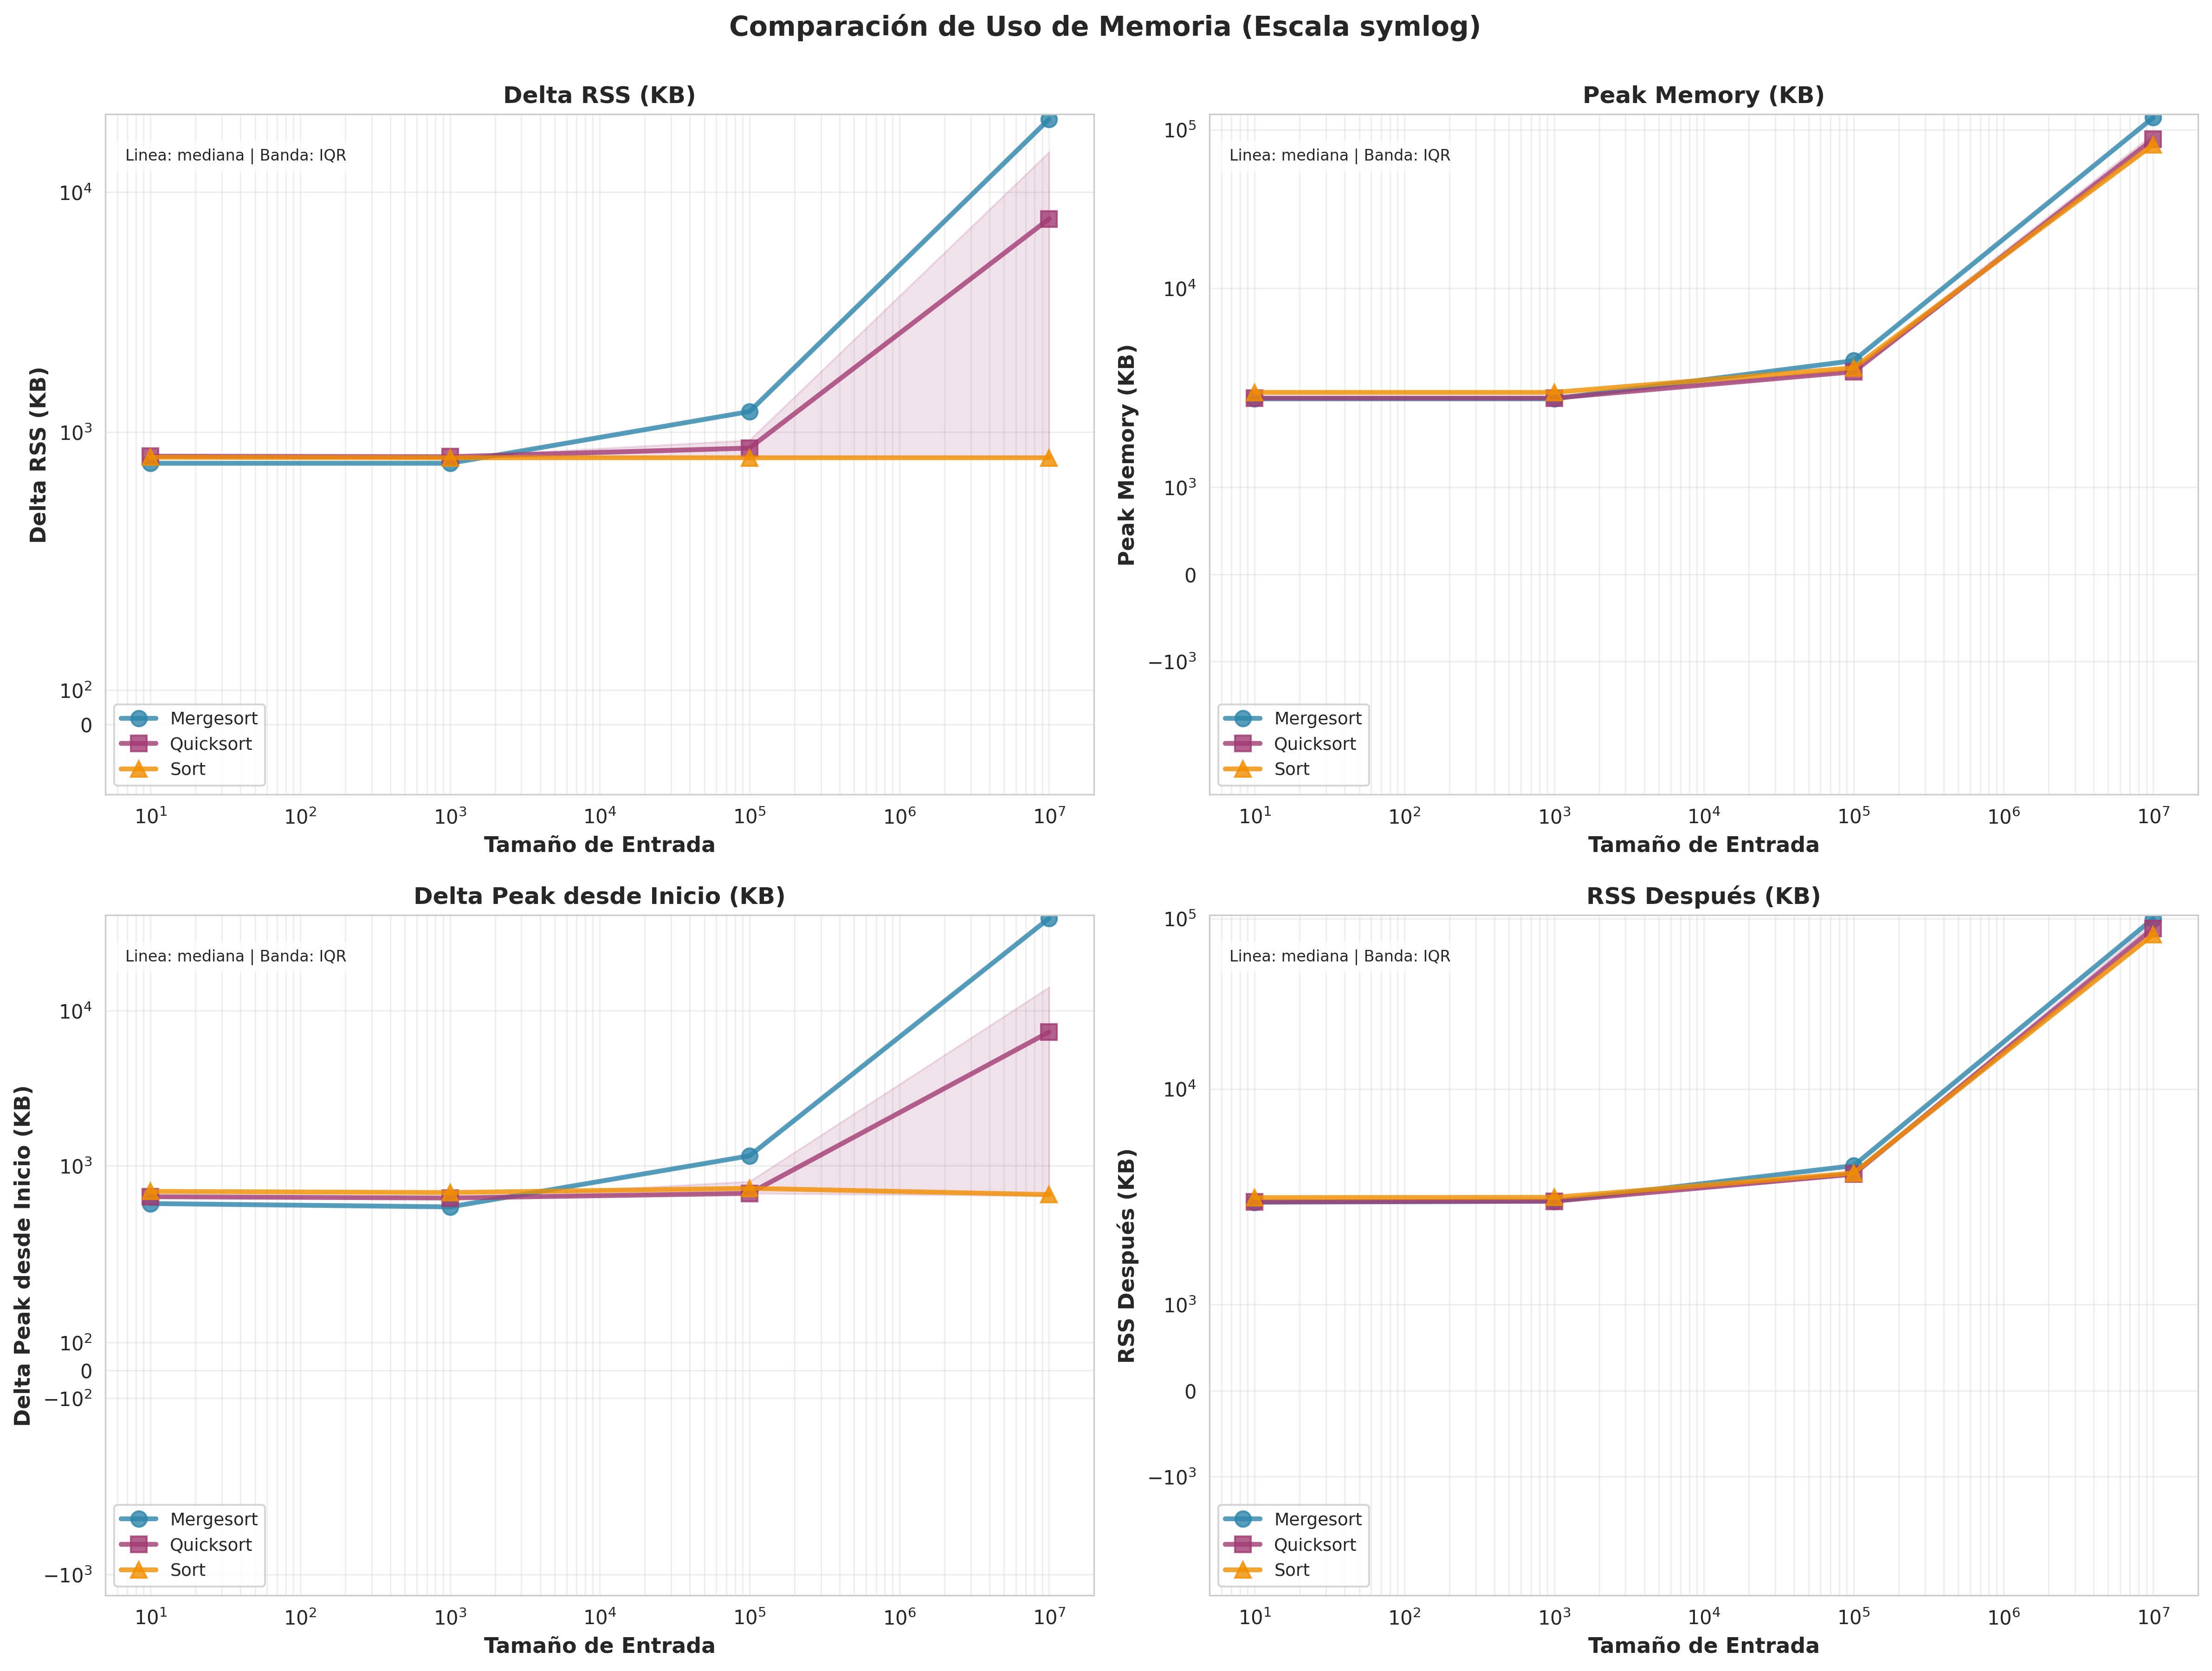
\includegraphics[width=\textwidth]{../code/sorting/data/plots/03_memoria_vs_tamaño.png}
    \caption{Todos los algoritmos Sorts Memoria vs Tamaño.}
\end{figure}

Primero, al observar \textit{Peak Memory} y \textit{RSS Después}, los tres algoritmos parecen bastante parecidos en tamaños pequeños y medianos. Entendemos esto porque estas métricas incluyen un costo inicial de importar librerías y funciones para medir su rendimiento. En otras palabras, para entradas pequeñas, el costo fijo domina y oculta diferencias finas entre algoritmos.

Segundo, cerca de $10^5$ y $10^7$, se pueden observar cambios notables donde los algoritmos empiezan a diferenciarse entre sí. Esto se debe a la forma que asignan la memoria, generando aumentos no lineales.

Ahora, \textbf{comparando algoritmo por algoritmo} en (\textit{Delta RSS} y \textit{Delta Peak desde Inicio}), se aprecia mejor el comportamiento real:

\begin{itemize}
    \item \textbf{Merge Sort} tiende a requerir más memoria adicional en tamaños grandes porque necesita arreglos temporales para combinar sublistas. Este comportamiento es esperado por su diseño, ya que no es in-place.

    \item \textbf{Quick Sort} es eficiente en memoria por ser in-place, pero tiene el riesgo de caer en recursión profunda en ciertos casos (por ejemplo, por una mala elección de pivote). Esto puede aumentar el consumo de stack y provocar problemas como \textit{Segmentation Fault} en tamaños muy grandes.

    \item \textbf{Sort} de C++ (Introsort) se mantiene como la alternativa más estable en la práctica: conserva buena eficiencia temporal y su uso de memoria adicional es contenido, gracias a que combina Quick Sort, Heap Sort e Insertion Sort según el caso.
\end{itemize}

A continuación, se presenta el análisis para los algoritmos de multiplicación de matrices.

\subsection*{Algoritmos de Multiplicación de Matrices}

\subsubsection*{Análisis de Tiempo}

Aquí los resultados obtenidos Tiempo (ms) vs Tamaño de la entrada N. Los datos de Tamaño son $\{2^4, 2^6, 2^8, 2^{10}\}$.

\begin{figure}[H]
    \centering
    \begin{minipage}[t]{0.49\textwidth}
        \centering
        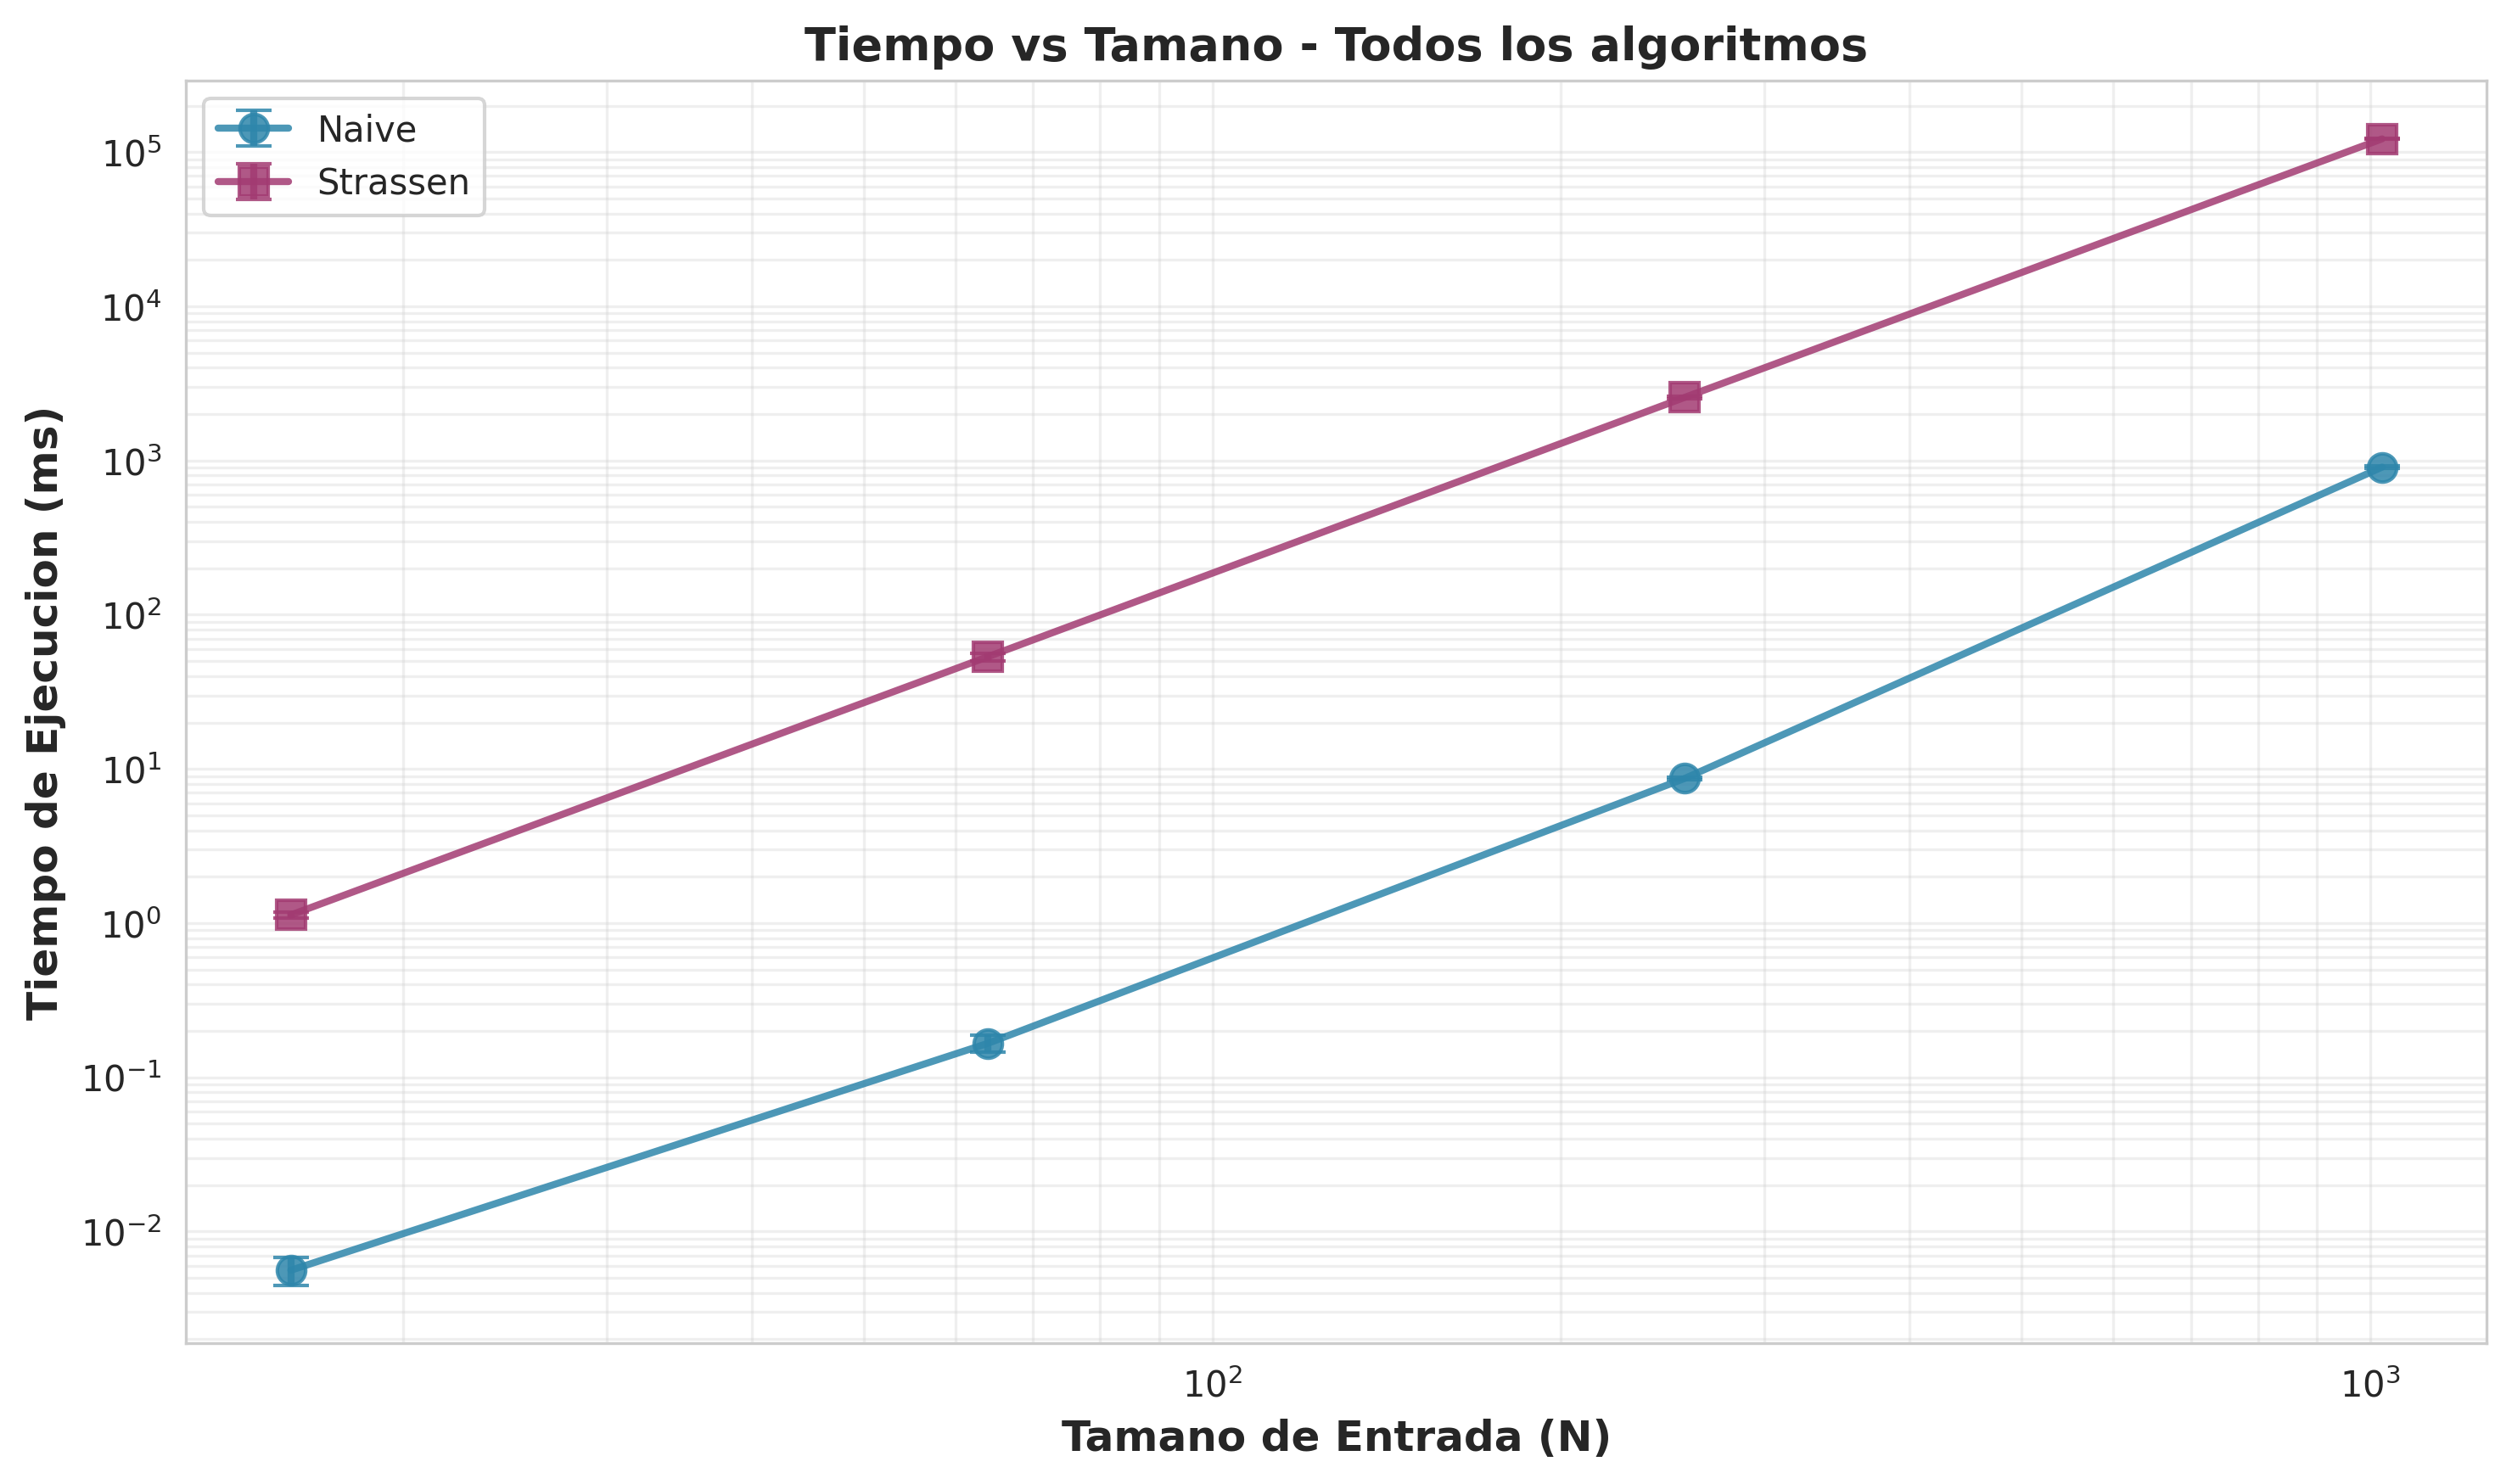
\includegraphics[width=\textwidth]{../code/matrix_multiplication/data/plots/01_tiempo_vs_tamano.png}
        \caption{Todos los algoritmos de Multiplicación.}
        \label{fig:matrix_todas}
    \end{minipage}
\end{figure}

En la \textbf{Figura 3} podemos observar los datos obtenidos de los algoritmos Naive y Strassen al intentar multiplicar matrices cuadradas de tamaños $\{2^4, 2^6, 2^8, 2^{10}\}$. Podemos observar que, aunque el algoritmo Naive tiene un tiempo de ejecución de $O(n^3)$ y Strassen tiene una complejidad de $O(n^{log_2 7})$, Naive sigue siendo superior al algoritmo Strassen en todo momento, incluso viendo después del tamaño $2^{10}$ aún se puede observar en el gráfico que Strassen es peor que Naive. Nos encontramos en una situación bizarra en donde el algoritmo con peor complejidad teórica es mejor en la práctica.

Por otro lado, tenemos al algoritmo \textbf{Strassen}, que en teoría debería ser mejor que \textbf{Naive}, ya que su tiempo de ejecución es de $O(n^{log_2 7})$. Además, al tener que hacer muchas operaciones con matrices temporales, el consumo de memoria es mucho mayor.

\textbf{¿Pero por qué sucede esto?} Después de analizar lo que estaba sucediendo, llegué a la conclusión que el algoritmo de Strassen puro es ineficiente para matrices pequeñas, y por esto mismo termina siendo peor en todo momento que Naive, ya que utiliza Strassen en todo momento sin importar el tamaño de la matriz. Una mejor implementación de Strassen debería utilizar Naive para matrices pequeñas, y Strassen para matrices grandes, ya que Strassen tiene una sobrecarga mayor por la cantidad de operaciones adicionales que debe realizar, además que se podría repartir la tarea en múltiples hilos del procesador para aprovechar mejor los CPUs modernos.
De esta manera se entiende que Strassen es mejor algoritmo cuando las matrices son muy grandes y su implementación es conjunto a Naive.

\subsubsection*{Análisis de Memoria}

En el análisis de memoria para multiplicación de matrices también se consideran cuatro métricas: \textit{Delta RSS}, \textit{Peak Memory}, \textit{Delta Peak desde Inicio} y \textit{RSS Después}.

\begin{figure}[H]
    \centering
    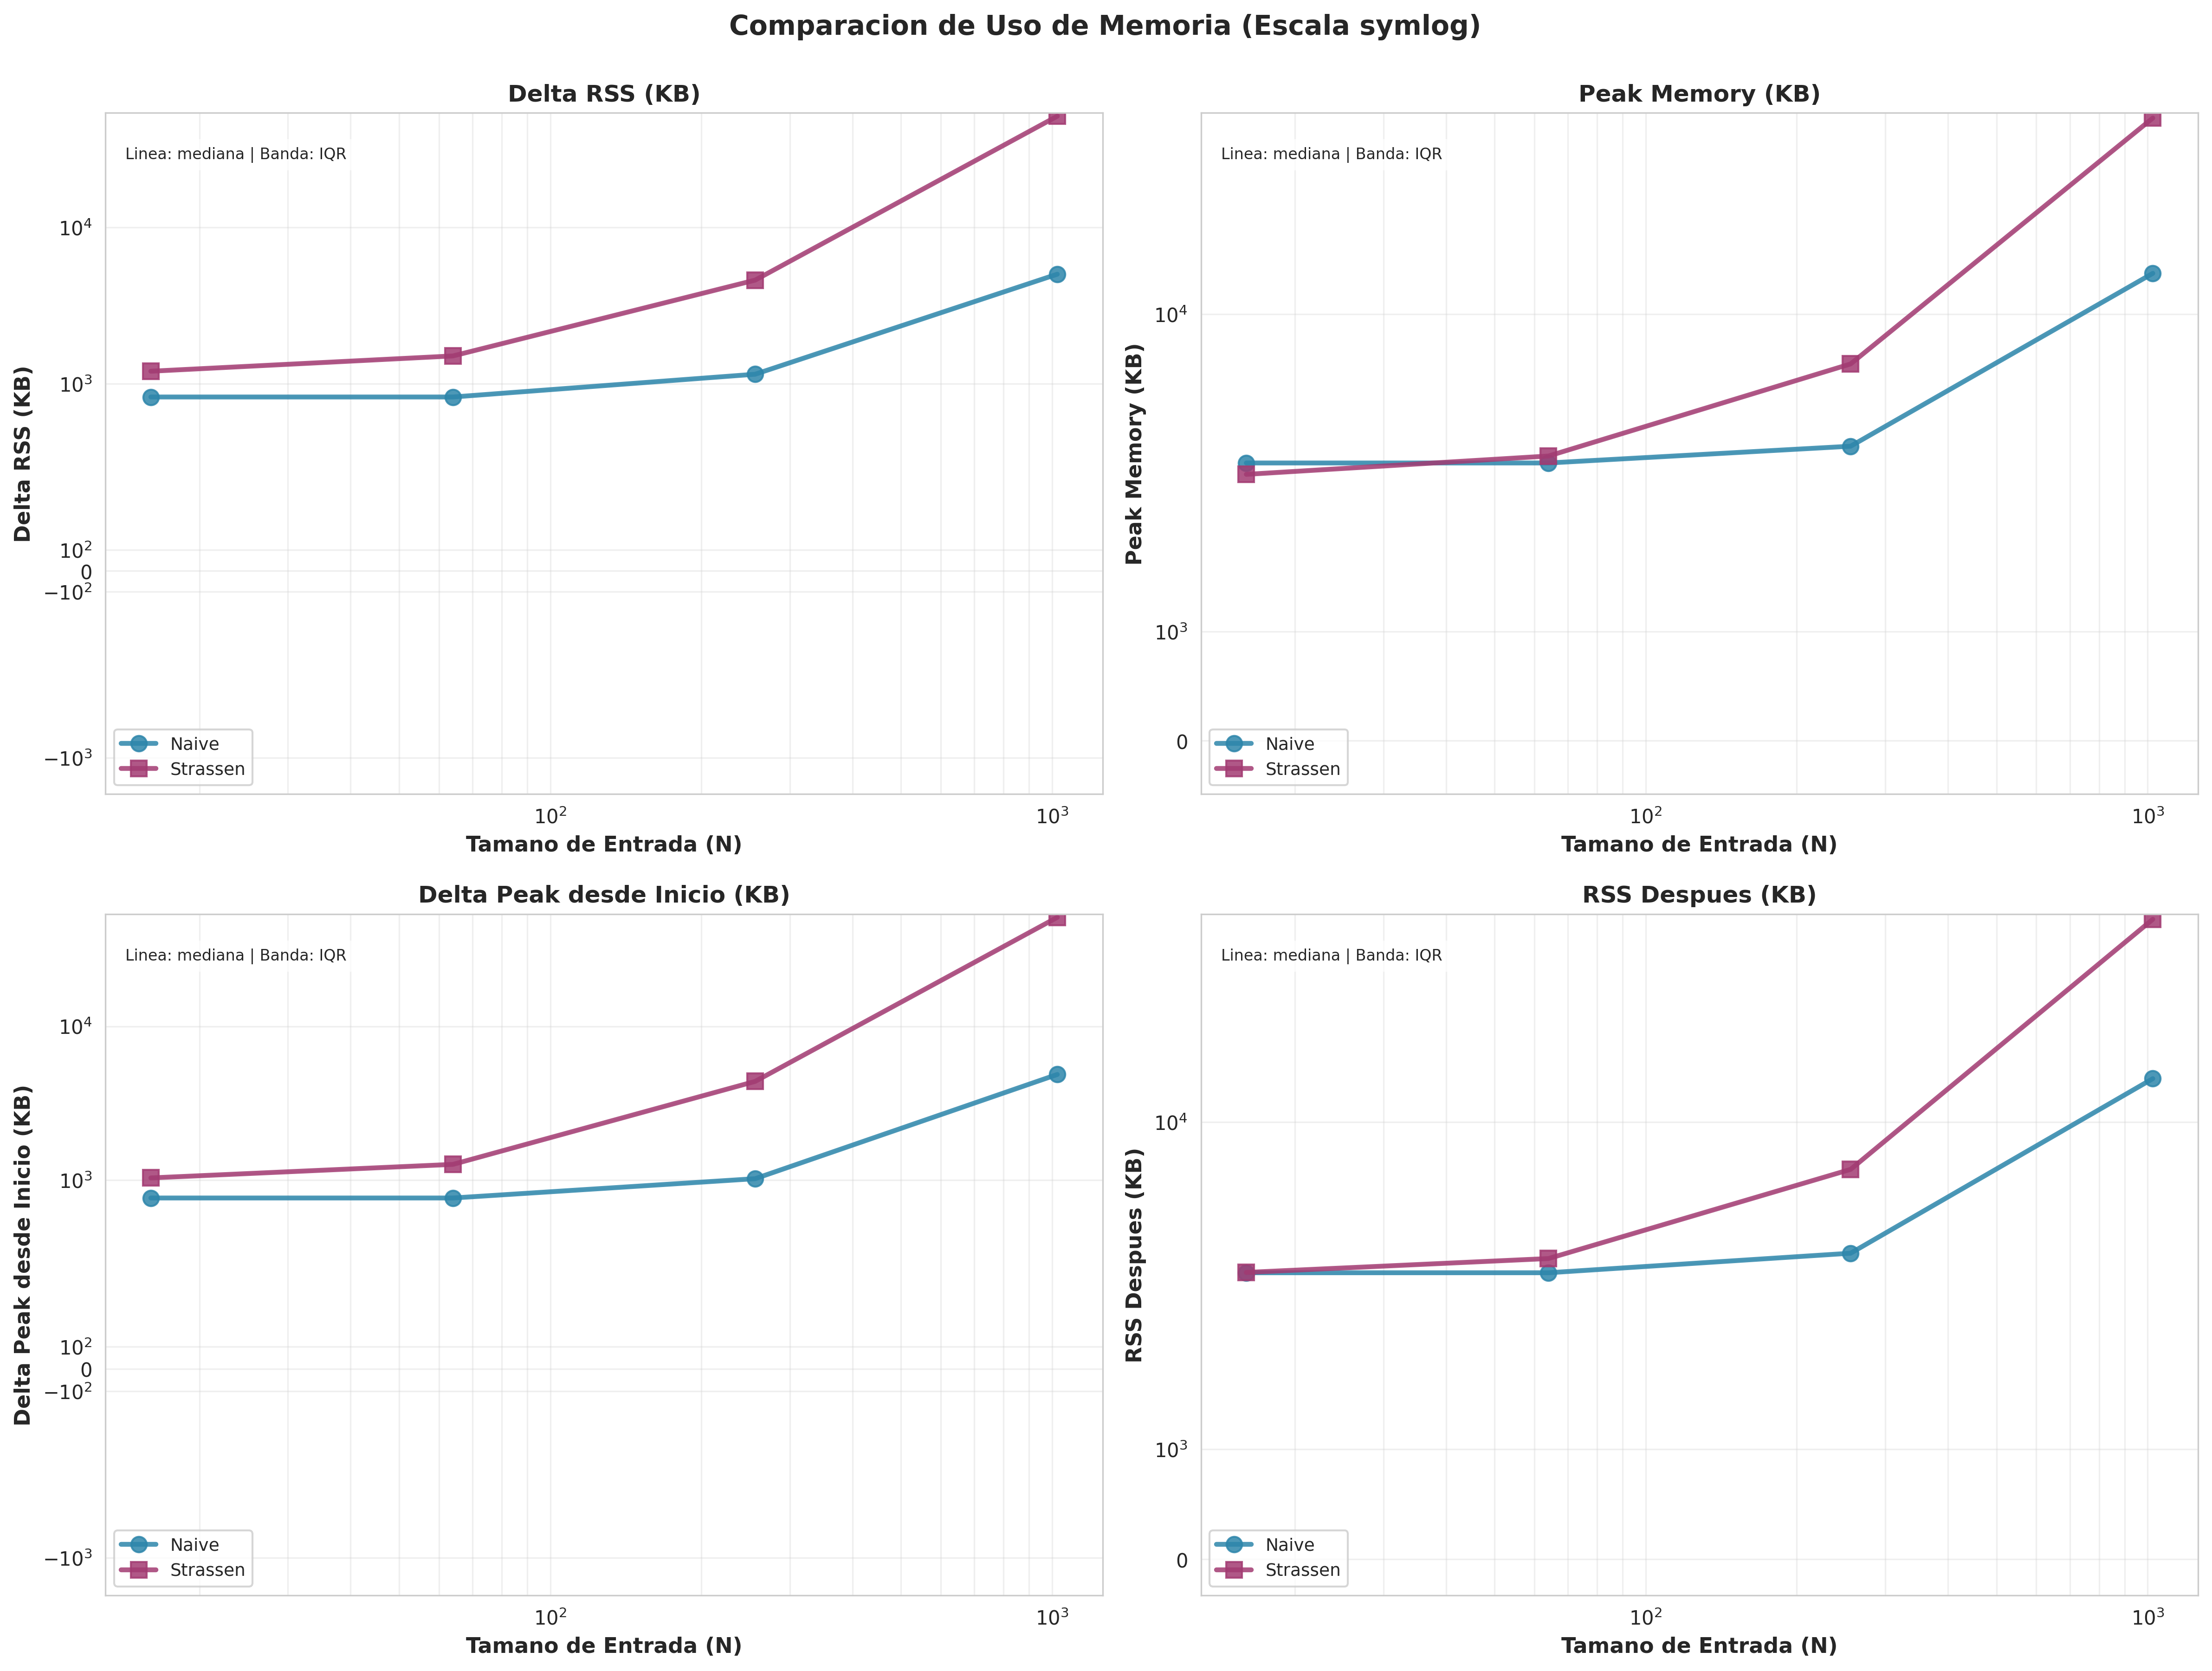
\includegraphics[width=\textwidth]{../code/matrix_multiplication/data/plots/05_memoria_vs_tamano.png}
    \caption{Uso de memoria en multiplicación de matrices (Naive vs Strassen).}
\end{figure}

Primero, en \textit{Peak Memory} y \textit{RSS Después} se aprecia que ambos algoritmos aumentan su consumo al crecer el tamaño de entrada, con saltos más notorios en los tamaños grandes. Este comportamiento se esperaba porque, además de la memoria de datos, el proceso arrastra costos de runtime, allocator y reservas de memoria.

Segundo, al observar las métricas (\textit{Delta RSS} y \textit{Delta Peak desde Inicio}), se nos muestra muy claramente el problema: Strassen requiere más memoria adicional que Naive, esto se nota especialmente para tamaños grandes. Esto coincide con la teoría y con la implementación práctica, ya que Strassen recursivamente crea múltiples submatrices temporales y realiza más operaciones intermedias durante la recursión.

Naive, en cambio, muestra un patrón más estable en la alocación de memoria. Aunque su complejidad temporal sea $O(n^3)$, su estructura de cálculo es más directa sin cálculos redundantes y con menos sobrecarga de estructuras auxiliares en comparación de Strassen que usa Dividir y Conquistar.

Se observa de Strassen una de las maneras más comunes para compensar la rapidez: el aumento del uso de la memoria con la complejidad temporal  ($O(n^{\log_2 7})$). En este caso, como el algoritmo no implementa Strassen de forma híbrida, su costo de memoria termina empeorando su rapidez.

En conclusión, se entiende que sin una implementación inteligente de Strassen, será como un tiro de la culata al final de cuentas, para estos tamaños y esta implementación, Naive simplemente es mejor en práctica en tiempo y memoria. Strassen mantiene su potencial para escalas matrices mayores cuando se implementa de manera híbrida (Strassen y Naive combinados). 

